\chapter{Quantum Mechanics} \label{ch:qm}

\section{State Vectors and Dirac Notation}

In quantum mechanics everything knowable about the state of some system is described in a vector, known as the state vector. The vector is from a vector space defined over the field of complex numbers, so it is important to use the correct definition of the inner product (§\ref{sec:vectors-complex}) where we take the conjugate of one of the vectors, to ensure that the inner product of a vector with itself is a non-negative a real number.

The inner product in this context is written like this:

$$\langle a|b \rangle$$

If the vectors $\vec{a}$ and $\vec{b}$ are represented by column matrices $a$ and $b$ (to spare ourselves, for the moment, from things we can't imagine, let's pretend we're discussing a finite-dimensional vector space), the above is equivalent to conjugate-transpose of $a$, written as $a^{\dagger}$ ("a-dagger"), matrix-multiplied by $b$:

$$a^{\dagger} \, b$$

We can split this inner product notation into separate pieces, so we can write $\langle a|$ to mean the vector whose matrix representation in some basis is a single row containing the complex conjugates of the elements in the single column of the matrix representing $|a \rangle$ in the corresponding dual basis.

Or more simply, $\langle a|$ is the covector of $|a \rangle$. The convention is therefore to think of $\langle a|$ as a function that extracts the coordinate of a basis vector $|a \rangle$ from its argument, which will be some vector $|b \rangle$, as in the expression $\langle a|b \rangle$. And in concrete matrix terms we can picture $\langle a|$ as a 1-row matrix (a row vector) that is the dual of the 1-column matrix (column vector) $|a \rangle$, and their corresponding coordinates are mutually complex conjugates.

And with this in mind, it follows that we can write them the other way round from the inner product:

$$|b \rangle \langle a |$$

which must therefore define a matrix: the product of a column vector on the left and a row vector on the right. This is the \textit{outer} product. A matrix can act as a vector-valued function of vectors: apply it to a vector to transform that vector to another vector. So:

$$|b \rangle \langle a | c \rangle$$

See how the notation nicely suggests we bracket the $\langle a | c \rangle$ first as an inner product and thus a mere number. So we immediately know that the result will be the vector $|b \rangle$ scaled by a number, i.e. it will be co-linear with $|b \rangle$. We've measured $|c \rangle$ against $|a \rangle$ and used that to scale $|b \rangle$.

Given an orthonormal basis $|b_n \rangle$, we can picture it as a set of $n$ column vectors, and expressed in their own basis they would be the standard basis. The outer product:

$$|b_n \rangle \langle b_n |$$

will produce a matrix with a single $1$ in one place of the diagonal. So if we sum over all $n$, we get the identity matrix, a matrix that makes no difference to whatever vector it applies to. Spelling this out, if our vector space has just two basis vectors:

$$|0 \rangle = \begin{bmatrix} 1 \\ 0 \end{bmatrix}$$

and

$$|1 \rangle = \begin{bmatrix} 0 \\ 1 \end{bmatrix}$$

Then the outer product of $|0 \rangle$ with itself is just:

$$
|0 \rangle \langle 0| = 
\begin{bmatrix} 1 \\ 0 \end{bmatrix}
\begin{bmatrix} 1 & 0 \end{bmatrix} =
\begin{bmatrix} 1 & 0 \\ 0 & 0 \end{bmatrix}
$$

and likewise of $|1 \rangle$ with itself:

$$
|1 \rangle \langle 1| = 
\begin{bmatrix} 0 \\ 1 \end{bmatrix}
\begin{bmatrix} 0 & 1 \end{bmatrix} =
\begin{bmatrix} 0 & 0 \\ 0 & 1 \end{bmatrix}
$$

And as predicted, summing those matrices gives the identity matrix:

$$
\begin{bmatrix} 1 & 0 \\ 0 & 0 \end{bmatrix} +
\begin{bmatrix} 0 & 0 \\ 0 & 1 \end{bmatrix} =
\begin{bmatrix} 1 & 0 \\ 0 & 1 \end{bmatrix}
$$

Even if the $|b_n \rangle$ were expressed in some other basis, the above summation would still be the identity matrix. Now for any vector $|c \rangle$ we can construct for each $n$:

$$|b_n \rangle \langle b_n | c \rangle$$

The $|b_n \rangle \langle b_n|$ operator is called a projection operator, because it projects its argument onto the subspace spanned by $|b_n \rangle$, resulting in a component vector of the argument in the direction of $|b_n \rangle$. Clearly if we act with the same projection operator again on that result, nothing will change, because it's already projected. This is a way of defining a projection operator: it's idempotent.

And the sum of all those resulting vectors for all $n$ will just be $|c \rangle$, of course, because we've done the equivalent of acting with the identity operator.

\section{Hilbert Spaces}

The vector spaces used to represent physical states are examples of Hilbert spaces, which is a category that includes most of the familiar examples (e.g. a simple Euclidean vector space is also a Hilbert space). A Hilbert space is an inner product space with certain requirements, but they are very loose requirements, so it also includes more exotic situations than we encounter elsewhere in physics:

\begin{itemize}
  \item scalars may be complex,
  \item despite which, there is an inner product that we can use to get a non-negative real number for the modulus of a vector: $\sqrt{\langle a|a \rangle}$, and 
  \item the space may be infinite dimensional.
\end{itemize}

The latter possibility includes infinities that are continuous (uncountable). Such vectors cannot be represented by a column of discrete values, not even an infinitely long column. Instead we have to specify a complex-valued function over a continuous (real) variable. Such functions can be added and scaled, as is required of a vector (§\ref{ch:linearity}) and so they qualify as elements of a vector space (§\ref{sec:vectors-space}) and we therefore have no choice but to admit that they are vectors.

The real parameter of such a function is analogous to the integer index that labels the rows in a column vector; instead of fetching the $i$th component by its position in the column, we evaluate the function with some real value $x$ to get its component "at" $x$.

Similarly, whereas the inner product over discrete components is:

$$
\langle a | b \rangle
=
\sum_i
x_i^* y_i
$$

the inner product over functions $f$ and $g$ of a real variable $x$ is:

$$
\langle f | g \rangle
=
\int_{-\infty}^{+\infty}
f(x)^* g(x)
dx
$$

This is also called the overlap integral, because it measures the extent to which the two functions overlap, but it is most definitely also the inner product between two vectors. Thus we can in some sense find the square of the "length" of a function: $\langle f | f \rangle$. This sounds like gibberish, but it is an unavoidable consequence of the definition of a vector space, which is abstract enough to admit a space of possible functions.

\section{Physical Interpretation}

To interpret the state vector physically, we choose a basis so we can resolve it into components. Our choice of basis has to do with the observable quantity we are presently interested in, such as position, momentum, orientation or energy. If it may take on any real value, the state vector will have to be a function of that value; if it may only take on certain discrete values, it can be a column vector (albeit sometimes one with infinitely many rows) in which each row corresponds to one of those possible discrete values that the observable may exhibit when measured.

The information available from the state vector is, in general, probabilistic. Each component, being a complex number, is related to the probability of the observable quantity taking on the value represented by that component. The squared modulus of the component (its value multiplied by the complex conjugate of its value) is the probability of obtaining that value, or if the state vector is a function $f(x)$, then:

$$\int_{a}^{b} f(x)^* f(x) \, dx$$

is the probability that $x$ will have a value somewhere between $a$ and $b$.

As a probability is a number between $0$ and $1$, it must be the case that the sum of the squared modulus of all the components (or the above integral from $-\infty$ to $+\infty$) must be $1$. This is the same as saying that $\langle S | S \rangle = 1$ for any physically realistic state vector. Or to put it another way, the magnitude of a state vector is not significant, only the direction (i.e. the relative values of the components in some basis). We will always fix the magnitude to be $1$.

Unsurprisingly, if one of the components is $1$ and all the others are zero, the vector represents certainty that the observable has the value represented by that component. But this also means that the state vector is equal to one of the basis vectors. Thus the basis vectors for an observable represent exact values that the observable may exhibit when measured.

Further, a measurement of the observable (or more precisely, any interaction producing subsequent behaviour that could be used to infer the value of the observable) causes the state vector to change to the basis vector of that observable corresponding to the measured value. This change is (at least in this theory) assumed to be instantaneous and to have no mechanism that we can deduce anything further about.

Thus after measuring an observable, subsequent measurements of the same observable will with certainty produce the same result.

(This is not quite true in the continuous cases when the state vector is actually a function of a real variable. We don't expect to ever find such a system precisely aligned with a single base state, but instead to have at least some small spread of probabilities.)

\section{Switching Basis}

Having constructed a column representation of a state vector in one basis, relating to one observable, we can switch to another. The operation for doing this will depend on both the "before" and "after" bases (§\ref{sec:vectors-change-basis}). A state vector contains everything knowable about a system, including all we can know about any of its observable quantities. By re-expressing the same state vector as a different set of components in terms of the basis associated with a different observable, we recover the probability distribution for that observable.

As always when using an operator to transform a vector's components we need to be clear on whether we want to get a different vector in the same basis or the same vector in a different basis. In this case, physically we're talking about the latter; a state vector represents something physically real, and we're just changing how we describe it. On the other hand, mathematically all we have is the description, and the choice of basis is not entirely arbitrary because a basis relates to an observable quantity.

An operator used to switch to another basis must preserve the inner product (and thus the lengths of, and angles between, vectors). This means it must be a \textit{unitary} operator, $\hat{U}$, for which the Hermitian conjugate serves as the inverse:

$$\hat{U} \hat{U}^\dagger = I$$

\section{Operators Representing Observables} \label{sec:qm-operators1}

Observables have an associated operator. Note that this is \textit{not} the same as the operator for converting a state vector to a different basis. In QM when we talk about the observable's associated operator, we are talking about something that is not directly of any use for converting between bases (it is not unitary, for one thing), though it will indicate how we could perform such an operation.

An observable operator can be applied to a state vector as a kind of test, but it is much more powerful when we picture it applying to every possible state vector (that is, all unit vectors in the space) to find out how it affects them.

In QM operators associated with observables are Hermitian or self-adjoint, meaning that for an operator $\hat{O}$:

$$\langle a|\hat{O} b \rangle = \langle \hat{O} a| b \rangle$$

This has a few useful implications:

\begin{itemize}
  \item in the discrete finite vector case, operators can be represented as a matrix $O$, $O^{\dagger} = O$, or $O_{ij} = O_{ji}^*$, so the main diagonal elements are real,
  \item regardless of representation, eigenvectors (§\ref{sec:vectors-eigen}) with distinct eigenvalues are orthogonal and complete (they span the space, so you can take a unit vector in each of these orthogonal directions and you have an orthonormal basis) and
  \item regardless of representation, their eigenvalues are real.
\end{itemize}

Think of the analogy of a Euclidean real plane vector space, and a symmetric $2 \times 2$ matrix $M$ operating on it. The eigenvectors are lines in the plane along which vectors do not change direction, only magnitude, when the operator is applied. Because the matrix is symmetric ($M_{ij} = M_{ji}$) these lines are orthogonal. So it is with an Hermitian operator in a complex space, with only the added complication of needing to be careful about taking the complex conjugate when comparing diagonally opposite elements.

The basis vectors of the observable are just unit vectors that are eigenvectors of the operator. That is, if you apply the observable's operator to every possible state vector, a subset of them will be scaled (by a potentially complex factor) without any change to their alignment. There will be a set of orthogonal unit vectors that pass this "alignment preserving" test, and these form the basis of the observable.

In other words, quantum mechanics is substantially about:

\begin{itemize}
  \item defining the operator for an observable,
  \item solving the eigenvalue equation for that operator (that is, finding its eigenvectors and their associated eigenvalues)
  \item using the eigenvectors as a basis for representing state vectors,
  \item assuming that when the observable is measured, the state will snap into alignment with one of those eigenvectors,
  \item interpreting a coordinate in that basis as a complex amplitude whose mod-square is the probability that the state will align itself with that basis vector,
  \item interpreting the eigenvalue associated with the basis vector as the measured value of the observable (the eigenvalues of Hermitian operators are real numbers, fortunately.)
\end{itemize}

If a system's state vector matches one of these eigenvectors, then the system is already in an eigenstate and if the observable is measured, the result will with certainty be the eigenvalue associated with that eigenstate.

Otherwise, the state vector will be a linear combination of the eigenstates, and if the observable is measured and found to have a particular value, then the state vector will have instantaneously realigned itself with an eigenvector having that eigenvalue.

It is therefore very clearly the case that an observable's operator should not be mistaken for a means to transform a state vector into the basis of the observable. Consider a state vector that is already aligned with an eigenstate of the operator, but is currently expressed as a linear combination of some other basis, so it has several non-zero coordinates. But in the basis of the observable, its coordinates should all be zero except for the eigenstate's coordinate, which will have some complex value of modulus $1$. The observable's operator clearly cannot bring about this transformation: the state vector's coordinates will all be scaled by the same factor (the eigenvalue), by the very definition of eigenvectors.

But if we solve the eigenvalue equation for the operator, we will know the complete basis of the observable, along with the eigenvalue associated with each basis vector, and we can then resolve our state vector against those basis vectors. Then we will have a set of coordinates that serve as probability amplitudes for the associated (measurable) eigenvalues.

In addition, there is a meaningful interpretation for the result of applying the operator for an observable to a given state vector: the inner product of that vector with the original state vector gives the expectation value (§\ref{ch:expectation}) of the observable.

While we've discussed all this in terms of more easily pictured finite-dimensional vectors with discrete complex components, all the same concepts translate to complex-valued functions of an integer or real parameter.

\section{The Wave Function}

One way to approach QM initially is to consider the position and momentum of an electron. These are continuous variables, so we will be working entirely with state vectors that are represented by functions of real variables, and operators that transform functions.

We model this situation as a continuous complex-valued function of position and time, $\Psi(x, y, z, t)$, very often abbreviated to $\Psi$. We will sometimes also consider functions only of space, $\psi$. (This upper/lowercase distinction is quite widespread but not universally observed.)

By considering only one spatial dimension we can picture the wave function at one instant as a line, somewhere along which the electron could be found. At each point $x$ on the line there is an associated complex plane (visualised as normal to the line), with an arrow lying in it, pointing out from the line. This is the complex value of $\Psi$ at that position $x$ and time $t$.

The complex plane should not be confused with vectors. Any given snapshot of $\Psi(x, t)$ at some instant $t$, given by a function $\psi(x)$, is itself an entire vector. The position $x$ labels a single infinitesimal component of the vector, and every such component is a complex number, which we can therefore visualise as a complex plane with an arrow on it.

So for example we could picture the arrows as making a corkscrew shape, rotating around the line such that the angle depends linearly on $x$, but the modulus of the complex value (the length of the arrow) happens to be constant in this example. This is the notional wave function for a free electron (no forces acting it) with a precisely defined momentum and therefore no defined position, something never observed in reality.

More generally, the arrow length will also vary with $x, t$. The arrow length at $x$ determines the likelihood that the electron will be found at $x$. More precisely, the modulus-squared of $\Psi$, which can be calculated with $\Psi^*\Psi$, is proportional to the probability density:

\begin{equation}
  \rho(x) = \Psi^*\Psi
  \label{eqn:pdf}
\end{equation}

Given the electron is in some region $A$ between $x_1$ and $x_2$, the integral:

$$
\alpha =
\int_{x_1}^{x_2}
\Psi^*\Psi
\,dx
$$

is \textit{proportional} to the probability of finding the electron in $A$.

Recall that the product of a complex number and its own complex conjugate is a real number, and here we are doing $\Psi(x)^*\Psi(x)$, using the single complex value at position $x$, so the result will be real. But the complex conjugate is not a general purpose magic way to get a real number from a product of any two complex numbers; $\Psi(x_1)^*\Psi(x_2)$ need not be real.

If we compute the same integral $\beta$ for some larger surrounding region $B$, we can compute the conditional probability:

$$
P(A|B) = \frac{\alpha}{\beta}
$$

That is: the probability of finding the electron in $A$ \textit{given that} it is somewhere in $B$ is given by the fraction $\alpha / \beta$.

If $\Psi$ is suitably behaved (square-integrable; roughly, it goes to zero at some distance and does not become infinite anywhere) then we can compute the integral over the whole of our one dimension of space:

$$
\alpha =
\int_{-\infty}^{+\infty}
\Psi^*\Psi
\,dx
$$

We can then include a factor of $1/\sqrt{\alpha}$ within $\Psi$ to "normalise" it, such that integrating the normalised $\Psi^*\Psi$ over some region will directly give us the absolute (unconditional) probability of finding the electron in that region.

Some interesting things to note at this early stage:

\begin{itemize}
  \item For the simple first example of the free electron with definite momentum, normalisation is not possible because the integral over all of space does not converge on a finite value.
  \item A global change in the amplitude of the function (scaling the entire function by some complex constant) is not a physically significant change; there is a set of wave functions $a\Psi$ for any complex constant $a$, which all mean the same thing. What matters is how the amplitude varies from place to place (the same will turn out to be true for the complex phase).
  \item To normalise, we have to find the sum over all space of the mod-squared wave function. Interpreting the wave function as a vector, we're taking the inner product of the vector with itself, so we are in a sense finding the "length"-squared of the wave function as a vector. We then can then use this factor to scale it to be a unit vector, but preserving the relative shape of the wave (that is, preserving the "alignment" of the vector).
\end{itemize}

\section{Schrödinger Equation}

Any wave can be described as a sum of many simple component waves. (It is interesting that we use the word "component"; they are also basis vectors, so in vector terminology we should use the word component to refer to the complex constant factor applied to each simple wave included in the sum).

Each individual component wave has \textit{two} parameters:

\begin{itemize}
  \item if we nominate a fixed point in space, there is a frequency of oscillation, $\nu$
  \item if we freeze time, we can measure the wavelength, $\lambda$, the distance between adjacent peaks in space
\end{itemize}

These can be independently adjusted (do not be confused by the familiar example of EM waves, where wavelength and frequency are coupled due to the constant speed of light!)

So the component wave can be described by the complex exponential:

$$
\Psi(x, t) = \exp \left[ 2\pi i(\frac{x}{\lambda} - \nu t) \right]
$$

Pick any fixed point in space, so $x$ is constant, and $\nu$ determines the rate of oscillation. Pick a fixed instant in time, so $t$ is constant, and $\lambda$ determines the distance between peaks. With both in play, we have a corkscrew complex wave pattern that is moving.

Anything we figure out for this model wave can be taken to be true for any linear combination of many such waves, in the sense that we can imagine decomposing some messy wave into a set of components, each component characterised only by two numbers.

Planck inferred the relationship between frequency and energy:

$$\nu = \frac{E}{h}$$

And de Broglie likewise for momentum and wavelength:

$$\lambda = \frac{h}{p}$$

So we can write the wave function very neatly in terms of energy and momentum instead:

$$
\Psi(x, t) = \exp \left[ {\frac{i(px - Et)}{\hbar}} \right]
$$

Nothing much has changed: as before, we have two parameters shaping a complex corkscrew wave. (We use $\hbar = h/2\pi$ for brevity because that combination isn't going away.) All that has changed is that we've got two parameters with a physical interpretation for something we've previously thought of as a "particle".

We can take the partial differential of the above w.r.t $t$ or $x$, and the way that works with exponentials is strangely illuminating.

Doing $t$ first:

$$
\frac{\partial \Psi}{\partial t}
=
-\frac{iE}{\hbar}
\exp \left[ {\frac{i(px - Et)}{\hbar}} \right]
$$

The constant factor is copied outside the exponential, which otherwise remains the same. So in fact:

$$
\frac{\partial \Psi}{\partial t}
=
-\frac{iE}{\hbar}
\Psi
$$

We can tidy up by multiplying both sides by $i\hbar$:

$$
i\hbar \frac{\partial \Psi}{\partial t}
= E \Psi
$$

The exact same procedure with $x$ yields:

$$
- i\hbar \frac{\partial \Psi}{\partial x}
= p \Psi
$$

But we can also take the second derivative and get:

$$
- \hbar^2 \frac{\partial^2 \Psi}{\partial x^2}
= p^2 \Psi
$$

Returning to our physical interpretation, a free particle has energy that is purely kinetic, related to its momentum by:

$$
p^2 = 2m E
$$

(This is just $\frac{1}{2}mv^2$ smushed into the definition of momentum, $mv$.)

Substituting the Planck and de Broglie relations:

$$
\frac{\hbar}{2m} = \lambda^2\nu
$$

In general a corkscrew wave is governed by two independent parameters:

\begin{itemize}
  \item momentum, which goes with wavelength (and the $x$ coordinate)
  \item energy, which goes with frequency (and the $t$ coordinate)
\end{itemize}

We've now coupled them, making them no longer independent. But we've also added a new parameter: the particle's mass. For a free particle of a given mass, if you know the momentum you know the energy, and vice versa. Equivalently, if you know the wavelength you know the frequency, and vice versa.

Returning to the classical relationship between momentum, energy and mass, we can use it to rewrite our expression for $p^2 \Psi$, substituting into the R.H.S. to easily obtain:

$$
- \hbar^2 \frac{\partial^2 \Psi}{\partial x^2}
= 2mE\Psi
$$

And as we also have an expression for $E\Psi$, let's isolate that:

$$
E\Psi =
- \frac{\hbar^2}{2m} \frac{\partial^2 \Psi}{\partial x^2}
$$

and insert our $E\Psi$ expression:

$$
i\hbar \frac{\partial \Psi}{\partial t}
=
- \frac{\hbar^2}{2m} \frac{\partial^2 \Psi}{\partial x^2}
$$

So, recalling that $\Psi$ is an abbreviation for $\Psi(x, t)$, a complex valued function of space and time, now we have a differential equation that relates only these things:

\begin{itemize}
  \item $\hbar$, Planck's constant, a universal fixed real number with units of joules-seconds, very accurately determined by experiment, not something we can adjust to fit this equation to different scenarios
  \item $i$, which just provides a 90\textdegree phase shift
  \item the first partial derivative of $\Psi$ w.r.t. to time, which is another function of space and time that tells you how $\Psi$ is changing
  \item $m$, the mass of the particle
  \item the second partial derivative of $\Psi$ w.r.t. space.
\end{itemize}

This means that from a snapshot $\psi$ (at a specific instant of time) of the wave function of a particle with a known mass, so you have its shape in space, you can find the second derivative of that shape w.r.t. space, then multiply that by $i\hbar/2m$ and you have the the first partial derivative of $\Psi$ w.r.t. to time. That is, a snapshot contains complete information about the past and future of the wave; it tells you how to compute every past and future state.

So far, so kind-of rigorous. The situation becomes vaguer when we introduce a force field acting on the particle.

Schrödinger himself seems to have mostly taken a guess and found that the resulting equation agreed with several previously unexplained experimental results. Many widely used textbooks don't even give any background for it but merely state it. More advanced theory can be used to derive it, e.g. it is a low-energy approximation of QED.

The full classical account of the energy of a particle is:

$$
E = \frac{p^2}{2m} + V
$$

where the potential is a function $V(x)$. Realistically it will also be a function of $t$, but later we're going to pretend it isn't.

Some authors note that by multiplying the above throughout by $\Psi$:

$$
E\Psi = \frac{p^2{\Psi}}{2m} + V{\Psi}
$$

we obtain some scaffolding into which we can plug in our expressions for $E \Psi$ and $p^2 \Psi$:

\begin{equation}
i\hbar \frac{\partial \Psi}{\partial t}
=
- \frac{\hbar^2}{2m} \frac{\partial^2 \Psi}{\partial x^2}
+ V{\Psi}
\label{eqn:se}
\end{equation}

And this is the same as the free particle equation with the added $V\Psi$ term, and is the complete Schrödinger equation which governs the time evolution of $\Psi$.

The extra term doesn't change the important property that if you have a snapshot $\psi(x)$ taken of $\Psi(x, t)$ at a specific initial instant of time, then you know all future states (glossing over what happens when there is any kind of interaction, including measurements).

This is sometimes contrasted with Newton's 2nd law relating acceleration to force, acceleration being the second order derivative of the position w.r.t time. Each time we integrate we need to conjure up a constant of integration, and we have to integrate acceleration twice to get the position. The two constants we need to add are the position and velocity. Thus a snapshot of the position of a particle is not generally enough to know what is happening to it.

But a snapshot $\psi(x)$ taken of $\Psi(x, t)$ at some time is not just one number, but a continuous function giving a (complex) number at each point $x$ along the line, so it is generously endowed with information. If we decompose the snapshot into component waves, each one has its own wavelength.

And if we multiple $\Psi$ by some constant (possibly complex) factor, the result is still a solution to the function. Such arbitrary constant scale factors make no difference to the physical meaning; what matters is how the function varies from location to location (and from time to time). This is what allows us to normalise the function (where possible) to ensure that it sums to 1 over all of space.

\section{Time Evolution}

We can say little here about wave functions unless they can be normalised, i.e. wave functions that tend to zero at infinity. Assuming this is the case, if we integrate the PDF over all of space:

$$
\int_{-\infty}^{+\infty}
\Psi^*\Psi
\,dx
$$

we expect the result to be constant (if normalised, it should always remain 1 as time passes), i.e.

$$
\frac{d}{d t}
\int_{-\infty}^{+\infty}
\Psi^*\Psi
\,dx
= 0
$$

Note that as we are integrating over $x$, outside the integral $x$ is not a variable. We can move the differentiation w.r.t. $t$ inside the integral, but only we change it to partial, because inside the integral $x$ is a variable:

$$
\int_{-\infty}^{+\infty}
\frac{\partial}{\partial t}
\Psi^*\Psi
\,dx
= 0
$$

Focusing on the inside of the integral, by the product rule:

$$
\frac{\partial}{\partial t} \, \Psi^*\Psi
=
\frac{\partial \Psi^*}{\partial t} \Psi
+
\frac{\partial \Psi}{\partial t} \Psi^*
$$

Now, the Schrödinger equation gives us an expression for the partial time derivative of the wave function by slightly rearranging \eqref{eqn:se}:

$$
\frac{\partial \Psi}{\partial t}
=
\frac{i \hbar}{2m} \frac{\partial^2 \Psi}{\partial x^2}
- \frac{i V}{\hbar}{\Psi}
$$

From this we can get the same for the complex conjugate:

$$
\frac{\partial \Psi^*}{\partial t}
=
- \frac{i \hbar}{2m} \frac{\partial^2 \Psi^*}{\partial x^2}
+ \frac{i V}{\hbar}{\Psi^*}
$$

Plugging those into our expression:

$$
\frac{\partial}{\partial t} \, \Psi^*\Psi
=
\left[
- \frac{i \hbar}{2m} \frac{\partial^2 \Psi^*}{\partial x^2}
+ \frac{i V}{\hbar}\Psi^*
\right] \Psi
+
\left[
\frac{i \hbar}{2m} \frac{\partial^2 \Psi}{\partial x^2}
- \frac{i V}{\hbar}\Psi
\right] \Psi^*
$$

Multiplying out:

$$
\frac{\partial}{\partial t} \, \Psi^*\Psi
=
- \frac{i \hbar}{2m} \frac{\partial^2 \Psi^*}{\partial x^2}
\Psi
+ \frac{i V}{\hbar}\Psi^*\Psi
+
\frac{i \hbar}{2m} \frac{\partial^2 \Psi}{\partial x^2}
\Psi^*
- \frac{i V}{\hbar}\Psi\Psi^*
$$

The second and fourth terms cancel each other:

$$
\frac{\partial}{\partial t} \, \Psi^*\Psi
=
- \frac{i \hbar}{2m} \frac{\partial^2 \Psi^*}{\partial x^2}
\Psi
+
\frac{i \hbar}{2m} \frac{\partial^2 \Psi}{\partial x^2}
\Psi^*
$$

Also there's a common factor we can pull out:

$$
\frac{\partial}{\partial t} \, \Psi^*\Psi
=
\frac{i \hbar}{2m}
\left[
\frac{\partial^2 \Psi}{\partial x^2}\Psi^*
- \frac{\partial^2 \Psi^*}{\partial x^2}\Psi
\right]
$$

Recall that we are working out an expression for this because it appears inside an integral over all space:

$$
\int_{-\infty}^{+\infty}
\frac{i \hbar}{2m}
\left[
\frac{\partial^2 \Psi}{\partial x^2}\Psi^*
- \frac{\partial^2 \Psi^*}{\partial x^2}\Psi
\right]
dx
$$

Now the fundamental theorem of calculus is that integration is the inverse of differentiation, so there is clearly some redundancy here in that we are taking the second partial differential w.r.t. $x$ only to then integrate over all $x$.

To make this explicit:

\begin{equation}  
\frac{\partial}{\partial t} \, \Psi^*\Psi
=
\frac{i \hbar}{2m} \
\left[
\frac{\partial}{\partial x}
\left(
\frac{\partial \Psi}{\partial x}\Psi^*
- \frac{\partial \Psi^*}{\partial x}\Psi
\right)
\right]
\label{eqn:qm-byparts}
\end{equation}

The integral and the partial differentiation w.r.t. $x$ cancel out to give us an expression that we can evaluate at the two limits and take the difference:

$$
\frac{d}{d t}
\int_{-\infty}^{+\infty}
\Psi^*\Psi
\,dx
=
\frac{i \hbar}{2m}
\left[
\frac{\partial \Psi}{\partial x}\Psi^*
- \frac{\partial \Psi^*}{\partial x}\Psi
\right]
\bigg\rvert_{-\infty}^{+\infty}
$$

If we do that, we will have an expression for the rate of change, w.r.t. to time, of the integral of $\Psi^*\Psi$ over all space.

But at these limits, we've said $\Psi$ goes to zero, so as to be normalisable, making the whole expression zero at those limits. So in fact we've shown that, as we wanted:

$$
\frac{d}{d t}
\int_{-\infty}^{+\infty}
\Psi^*\Psi
\,dx
= 0
$$

So if it is possible to normalise a wave function at all, and it satisfies \eqref{eqn:se}, then the constant of normalisation lives up to its name: it is the same for all time.

\section{Motion}

Given this abstract notion of an electron being entirely represented by a complex-valued function of position, how can we make sense of an electron moving?

Supposing the wave function is more concentrated in some region, it makes sense to compute the expectation value of the position variable:

$$
\langle x \rangle =
\int_{-\infty}^{+\infty}
x \, \rho(x)
\,dx
$$

Substituting our definition of $\rho$ from \eqref{eqn:pdf}:

$$
\langle x \rangle =
\int_{-\infty}^{+\infty}
x \, \Psi^*\Psi
\,dx
$$

remembering always that $\Psi$ is short for $\Psi(x, t)$, so $\langle x \rangle$ is also a function of $t$, and so this gives us a way of thinking about motion: the way the expectation value of the position changes with time.

$$
\frac{d}{dt} \langle x \rangle =
\frac{d}{dt}
\int_{-\infty}^{+\infty}
x \, \Psi^*\Psi
\,dx
$$

We can rearrange to move the derivative inside the integral, giving:

$$
\frac{d}{dt} \langle x \rangle =
\int_{-\infty}^{+\infty}
x \frac{\partial}{\partial t}
\, \Psi^*\Psi
\,dx
$$

Like before, it's the $t$-derivative of something that depends on $x$, inside the integral over $x$ we clarify that it is the partial derivative, and therefore $x$ is a constant for that derivative.

And borrowing from \eqref{eqn:qm-byparts} we can rewrite this as:

$$
\frac{d}{dt} \langle x \rangle =
\frac{i \hbar}{2m}
\int_{-\infty}^{+\infty}
x
\frac{\partial}{\partial x} \
\left(
\frac{\partial \Psi}{\partial x}\Psi^*
- \frac{\partial \Psi^*}{\partial x}\Psi
\right)
\,dx
$$

This isn't as simple as before where we cancelled out the integration and the differentiation, because of the pesky $x$. But the good news is this is the easiest ever opportunity for integration by parts. Recall:

$$
\int
u
\frac{dv}{dx}
dx = uv -
\int
v
\frac{du}{dx}
dx
$$

So $u$ is just $x$ and to get $v$ we have to calculate it at the limits:

$$
v =
\frac{\partial \Psi}{\partial x}\Psi^*
- \frac{\partial \Psi^*}{\partial x}\Psi
\bigg\rvert_{-\infty}^{+\infty}
$$

Plugging them in:

$$
x
\left(
\frac{\partial \Psi}{\partial x}\Psi^*
- \frac{\partial \Psi^*}{\partial x}\Psi
\right)
\bigg\rvert_{-\infty}^{+\infty}
-
\int_{-\infty}^{+\infty}
\left(
\frac{\partial \Psi}{\partial x}\Psi^*
- \frac{\partial \Psi^*}{\partial x}\Psi
\right)
\frac{dx}{dx}
dx
$$

As before, with $\Psi$ vanishing at infinity the first term can be removed, and of course $dx/dx$ is $1$. Finally the above is just the integral from our $\langle x \rangle$ expression, so:

$$
\frac{d}{dt} \langle x \rangle = -
\frac{i \hbar}{2m}
\int_{-\infty}^{+\infty}
\left(
\frac{\partial \Psi}{\partial x}\Psi^*
- \frac{\partial \Psi^*}{\partial x}\Psi
\right)
dx
$$

Having unwrapped one layer with integration by parts we can pull the same trick with $\frac{\partial \Psi^*}{\partial x}\Psi$, with $u = \Psi$ and $v = \Psi^*$, which once again means the $uv$ term is zero, leaving:

$$
-
\int_{-\infty}^{+\infty}
\frac{\partial \Psi}{\partial x}
\Psi^*
$$

So putting this back into $\langle x \rangle$:

$$
\frac{d}{dt} \langle x \rangle = -
\frac{i \hbar}{2m}
\int_{-\infty}^{+\infty}
\left(
\frac{\partial \Psi}{\partial x}\Psi^*
+ \frac{\partial \Psi}{\partial x}\Psi^*
\right)
dx
$$

The two identical terms cancel with the $2$ on the bottom of the fraction, so:

$$
\frac{d}{dt} \langle x \rangle = -
\frac{i \hbar}{m}
\int_{-\infty}^{+\infty}
\frac{\partial \Psi}{\partial x}\Psi^*
dx
$$

If we think of the rate of change of $\langle x \rangle$ as the expectation value of the velocity, or $\langle v \rangle$, we can multiply by $m$ to get $\langle p \rangle$, which actually cancels the $m$.

$$
\langle p \rangle = -
i \hbar
\int_{-\infty}^{+\infty}
\frac{\partial \Psi}{\partial x}\Psi^*
dx
$$

\section{Operators Again} \label{sec:qm-operators2}

Another way to describe what we're doing here is rediscovering operators. To apply an operator $\hat{O}$ and get its expectation value $\langle O \rangle$, the recipe is:

$$
\langle O \rangle =
\int_{-\infty}^{+\infty}
\Psi^*
\hat{O}
\Psi
\,dx
$$

How does this relate to our previous discussion about observable operators (§\ref{sec:qm-operators1})? We said that the operator for an observable is Hermitian, so it has orthogonal eigenvectors, and if the state vector is equal to an eigenvector then the observable, when measured, will be certain to equal the eigenvalue of that eigenvector. Our wave function at an instant in time $\psi(x)$ is a vector. To get a coordinate from that vector, we evaluate the function for some position $x$, and so the vector has a "coordinate" for every point in space. Therefore it is a vector expressed in the "position basis".

If the particle is very precisely localised, the function's value (the coordinates) will be zero everywhere except at that precise location. At the theoretical extreme, it will zero everywhere except at an infinitesimal single position (§\ref{sec:fourier-spike}). That is, it will be a basis vector in the position basis.

An observable operator has to scale its eigenvectors by the value that would be measured for a state equal to that eigenvector. That is exactly what happens if we multiply $\psi(x)$ by $x$: if it is a pure spike (a complex value of modulus $1$) at some position $x_1$, and zero everywhere else, the spike (and thus the whole vector) will be scaled by the value $x_1$. Whereas if it isn't a pure spike (not a position eigenvector), each non-zero value will be multiplied by a different value (its own position value), which will distort the shape of the function (or equivalently, change the "direction" of the vector).

We also mentioned in passing that if we apply an observable's operator to a specific state vector, we get an adjusted vector, and if we take the inner product between the original state vector and the adjusted vector, the resulting scalar value will be the expectation value of the observable. So this is just another way of writing down the above integral:

$$
\langle O \rangle =
\langle \Psi| \hat{O} | \Psi \rangle
$$

Because $\Psi$ is a function of $x$ and $t$, by integrating over all $x$ we get a function of time, telling us the evolving expectation value of whatever observable the operator represents. To remove a little complexity we'll switch to considering an instant of time so $\psi(x)$ is all we need.

This "operator sandwich" pattern is intuitively sensible when we apply the position operator to a wave function of position, because this fits precisely with how we understand the expectation value to be computed: it is the sum of every possible value multiplied by its probability of occurring. $\hat{x}|\psi\rangle$ is just $x \psi(x)$. If we multiply that by $\psi(x)^*$ then it will be $x$ multiplied by the probability of measuring the position to be $x$; clearly then the integral over all space will be the expectation value $\langle x \rangle$.

So in the position basis, the position operator $\hat{x}$ is just $x$ itself:

$$
\langle x \rangle =
\int_{-\infty}^{+\infty}
\psi(x)^*
\hat{x}
\psi(x)
\,dx
=
\int_{-\infty}^{+\infty}
\psi(x)^*
x
\psi(x)
\,dx
$$

The momentum operator $\hat{p}$, which we discovered above by looking for the expectation value of momentum, is $-ih\frac{\partial}{\partial x}$:

\begin{equation}
\begin{split}
  \langle p \rangle &=
  \int_{-\infty}^{+\infty}
  \psi(x)^*
  \hat{p}
  \psi(x)
  \,dx 
  \\
  &=
  \int_{-\infty}^{+\infty}
  \psi(x)^*
  (-ih\frac{\partial}{\partial x})
  \psi(x)
  \,dx 
  \\
  &= -ih
  \int_{-\infty}^{+\infty}
  \psi(x)^*
  \frac{\partial \psi(x)}{\partial x}
  \,dx  
\end{split}
\end{equation}

Compared to the position operator, it is somewhat less obvious what the momentum operator is doing to produce an expectation value for momentum. The intuitive process would be to sum (over all possible momenta) the product of each momentum and its probability of being measured. That would seem to require a wave function of momentum instead of position, and an integral over all momenta. And yet here we still have an integral over all positions, involving a wave function of position. \textit{We have not yet changed basis.}

To represent a vector as a set of coordinate in some basis, we extract each coordinate of the vector by performing the inner product between the unit basis vector for that coordinate and the vector in question. But for these functions of real parameters like position and momentum, the definition of a vector (that is, the set of its coordinates) is given by a function of the real parameter, the values of that function being the coordinates, each coordinate labelled with the real parameter, and the inner product is an integral over all values of the real parameter.

Momentum basis vectors in the position basis are of the form:

$$
\phi(x) = \frac{1}{\sqrt{2\pi\hbar}}e^{ipx/\hbar}
$$

That is, they are a function of position (we're still in the position basis, so the "components" of the vector are labelled by positions), but there is a momentum variable $p$ in the definition. That value of $p$ determines which basis vector of momentum this $\phi(x)$ describes.

The inner product of this with our state vector $\psi(x)$ (which is also expressed in the position basis) is the integral:

$$
\int_{-\infty}^{+\infty}
\psi(x)^*
\frac{1}{\sqrt{2\pi\hbar}}e^{ipx/\hbar}
\,dx
$$

This yields a single complex number that is the "coordinate" associated with momentum $p$ of our state vector in the momentum basis. So the complete description of our state in the momentum basis is a function of momentum:

$$
\psi(p) = \int_{-\infty}^{+\infty}
\psi(x)^*
\frac{1}{\sqrt{2\pi\hbar}}e^{ipx/\hbar}
\,dx
$$

Multiplying by a complex exponential inside an integral in this way is recognisable as the Fourier transform. But also, now we have $\psi(p)$ we can get the expectation value of momentum in exactly the same way as we did for position: by integrating (over all momenta) $\psi^* \hat{p} \psi(p)$:

$$
\langle p \rangle =
\int_{-\infty}^{+\infty}
\psi(p)^*
\hat{p}
\psi(p)
\,dp
$$

In the momentum basis, the $\hat{p}$ operator is just multiplying by $p$ (exactly like the position operator in the position basis.)

$$
\langle p \rangle =
\int_{-\infty}^{+\infty}
\psi(p)^*
p
\psi(p)
\,dp
$$

And $\psi(p)^*\psi(p)$ is the mod-square of the coordinate for $p$, that is, the probability that the momentum has the value $p$. 

The point is if we do change basis, we are not materially changing what is calculated. It is perhaps easier to comprehend this intuitively through the analogy with regular vectors, and by remembering that vectors are basis independent objects (§\ref{sec:vectors-geometric}). The observable operator acts on the state vector, in general changing both its length and alignment (unless the state vector happens to already be an eigenstate of the observable, in which case only the length changes). But this action would be the same regardless of the basis we are working in, and so it isn't necessary to get hung up on that point. Likewise, projecting the operated-on vector back on to the original state vector, to produce a scalar expectation value, is a geometrical, basis-independent operation. The inner product depends on the relative lengths and the angle between the two vectors. As long as when we change basis we do so in a way that preserves the inner product (that is, by a \textit{unitary} operator), then the choice of basis is physically irrelevant. 

Therefore, in this recipe for the expectation value, the operator $\hat{O}$, the state vector $| \psi \rangle$ and the adjusted vector $\hat{O} | \psi \rangle$ should all be understood as having an independent existence from any choice of basis:

$$
\langle \psi| \hat{O} | \psi \rangle
$$

That expression is a scalar value, and is the same regardless of the basis we work in (if we switch basis, we must use a unitary operator so the inner product between any two vectors is unaffected by the change of basis). When we want to calculate the value, we use the same basis throughout.

One way to visualise this is by simplifying radically, keeping to real numbers and two-dimensional Hilbert space, which is to say, the Euclidean plane, making it possible to draw pictures. A state $|\psi\rangle$ is a vector. \textit{It is not intrinsically in any basis.} But it is certainly of unit length.

\begin{figure}[h]
  \centering
    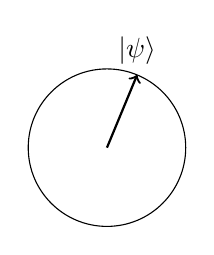
\begin{tikzpicture}
      \draw (0,0) circle (1);
      \draw[thick,->] (0,0) -- (0.383,0.924) node[anchor=south] {$|\psi\rangle$};
    \end{tikzpicture}
  \centering
  \caption{Anonymous state vector} \label{fig:state-vector}
\end{figure}

Suppose the system can be found to be in one of two moods, $|a\rangle$ (affable) and $|b\rangle$ (bored). These will correspond to two orthonormal state vectors:

\begin{figure}[h]
  \centering
    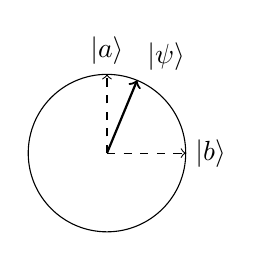
\begin{tikzpicture}
      \draw (0,0) circle (1);
      \draw[thick,->] (0,0) -- (0.383,0.924) node[anchor=south west] {$|\psi\rangle$};
      \draw[dashed,->] (0,0) -- (1,0) node[anchor=west] {$|b\rangle$};
      \draw[dashed,->] (0,0) -- (0,1) node[anchor=south] {$|a\rangle$};
    \end{tikzpicture}
  \centering
  \caption{Mood basis} \label{fig:mood-basis}
\end{figure}

Naturally $\psi$ can be resolved into pair of coordinates by using the orthonormal vectors of mood as a basis. We are tempted to say that the mood is presently more closely aligned with affable rather than bored, but must always remember that the mood can only ever be measured to be exactly affable or exactly bored (upon which it will snap into alignment with $|a\rangle$ or $|b\rangle$ accordingly). It is just more likely to found affable, with probability given by the square of the coordinate given by the inner product $\langle a|\psi \rangle$.

Also the system can be found to be listening to music in one of two genres, $|c\rangle$ (country) or $|d\rangle$ (disco):

\begin{figure}[h]
  \centering
    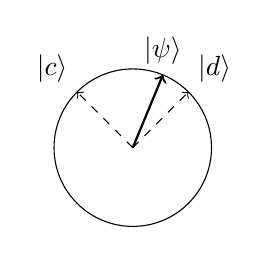
\begin{tikzpicture}
      \draw (0,0) circle (1);
      \draw[thick,->] (0,0) -- (0.383,0.924) node[anchor=south] {$|\psi\rangle$};
      \draw[dashed,->] (0,0) -- (-0.707,0.707) node[anchor=south east] {$|c\rangle$};
      \draw[dashed,->] (0,0) -- (0.707,0.707) node[anchor=south west] {$|d\rangle$};
    \end{tikzpicture}
  \centering
  \caption{Genre basis} \label{fig:genre-basis}
\end{figure}

Against this genre basis the coordinates for the same $|\psi\rangle$ are clearly going to be different from what they were in the mood basis, and our $|\psi\rangle$ is leaning more toward disco than country. If you tilt your head to the left\footnote{That is, apply a unitary operator} so as to align $|d\rangle$ with the horizontal, pointing right, and $|c\rangle$ with the vertical, pointing up, then $|\psi\rangle$ will appear to be closer to horizontal than vertical.

Returning to the mood observable, there is an operator $\hat{M}$ associated with that observable. We can think of the operator as acting on all possible state vectors, represented by an evenly-spaced selection of them.

\begin{figure}[h]    
  \caption{Effect of operator $\hat{M}$}
  \begin{subfigure}{0.5\textwidth}
      \centering
      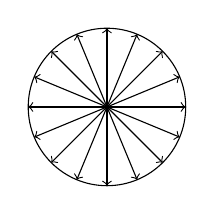
\begin{tikzpicture}
        \draw (0,0) circle (1);
        \draw[->] (0,0) -- (1.000,0.000);
        \draw[->] (0,0) -- (0.924,0.383);
        \draw[->] (0,0) -- (0.707,0.707);
        \draw[->] (0,0) -- (0.383,0.924);
        \draw[->] (0,0) -- (0.000,1.000);
        \draw[->] (0,0) -- (-0.383,0.924);
        \draw[->] (0,0) -- (-0.707,0.707);
        \draw[->] (0,0) -- (-0.924,0.383);
        \draw[->] (0,0) -- (-1.000,0.000);
        \draw[->] (0,0) -- (-0.924,-0.383);
        \draw[->] (0,0) -- (-0.707,-0.707);
        \draw[->] (0,0) -- (-0.383,-0.924);
        \draw[->] (0,0) -- (-0.000,-1.000);
        \draw[->] (0,0) -- (0.383,-0.924);
        \draw[->] (0,0) -- (0.707,-0.707);
        \draw[->] (0,0) -- (0.924,-0.383);
      \end{tikzpicture}
  \caption{Before} \label{fig:mood-before}
  \end{subfigure}
  \begin{subfigure}{0.5\textwidth}
      \centering
      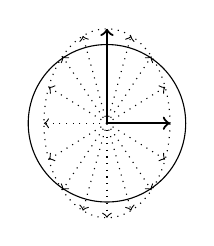
\begin{tikzpicture}
        \draw (0,0) circle (1);
        \draw[dotted] (0,0) ellipse (0.8 and 1.2);
        \draw[thick,->] (0,0) -- (0.800,0.000);
        \draw[dotted,->] (0,0) -- (0.739,0.459);
        \draw[dotted,->] (0,0) -- (0.566,0.849);
        \draw[dotted,->] (0,0) -- (0.306,1.109);
        \draw[thick,->] (0,0) -- (0.000,1.200);
        \draw[dotted,->] (0,0) -- (-0.306,1.109);
        \draw[dotted,->] (0,0) -- (-0.566,0.849);
        \draw[dotted,->] (0,0) -- (-0.739,0.459);
        \draw[dotted,->] (0,0) -- (-0.800,0.000);
        \draw[dotted,->] (0,0) -- (-0.739,-0.459);
        \draw[dotted,->] (0,0) -- (-0.566,-0.849);
        \draw[dotted,->] (0,0) -- (-0.306,-1.109);
        \draw[dotted,->] (0,0) -- (-0.000,-1.200);
        \draw[dotted,->] (0,0) -- (0.306,-1.109);
        \draw[dotted,->] (0,0) -- (0.566,-0.849);
        \draw[dotted,->] (0,0) -- (0.739,-0.459);
      \end{tikzpicture}
      \caption{After} \label{fig:mood-after}
  \end{subfigure}
\end{figure}

After the operator has done its work, the adjusted vectors fit into an ellipse rather than a circle: they are no longer all unit vectors. There are just two directions along which the vectors preserved their alignment: these are the eigenvectors of $\hat{M}$. They are orthogonal. This is how we discovered the basis vectors $|a\rangle$ and $|b\rangle$, by finding the states $|\psi\rangle$ for which:

$$
\hat{M}|\psi\rangle = m|\psi\rangle
$$

where $m$ is just a number, i.e. the directions along which $\hat{M}$ does not change the alignment of the vector, only the length. Also the scaling factor along (say) the $|b\rangle$ direction is the numerical measurement that we interpret as the bored state.

Operators associated with observables, such as $\hat{M}$, are Hermitian, which (in this real vector space with only two orthogonal directions) means they can be represented by a symmetric $2 \times 2$ matrix, and will always have the effect of stretching or squashing along two orthogonal directions, thus picking out the two basis vectors for the observable.

And to be complete we should visualise the effect of the genre operator $\hat{G}$.

\begin{figure}[h]    
  \caption{Effect of operator $\hat{G}$}
  \begin{subfigure}{0.5\textwidth}
      \centering
      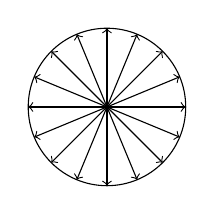
\begin{tikzpicture}
        \draw (0,0) circle (1);
        \draw[->] (0,0) -- (1.000,0.000);
        \draw[->] (0,0) -- (0.924,0.383);
        \draw[->] (0,0) -- (0.707,0.707);
        \draw[->] (0,0) -- (0.383,0.924);
        \draw[->] (0,0) -- (0.000,1.000);
        \draw[->] (0,0) -- (-0.383,0.924);
        \draw[->] (0,0) -- (-0.707,0.707);
        \draw[->] (0,0) -- (-0.924,0.383);
        \draw[->] (0,0) -- (-1.000,0.000);
        \draw[->] (0,0) -- (-0.924,-0.383);
        \draw[->] (0,0) -- (-0.707,-0.707);
        \draw[->] (0,0) -- (-0.383,-0.924);
        \draw[->] (0,0) -- (-0.000,-1.000);
        \draw[->] (0,0) -- (0.383,-0.924);
        \draw[->] (0,0) -- (0.707,-0.707);
        \draw[->] (0,0) -- (0.924,-0.383);
      \end{tikzpicture}
  \caption{Before} \label{fig:genre-before}
  \end{subfigure}
  \begin{subfigure}{0.5\textwidth}
      \centering
      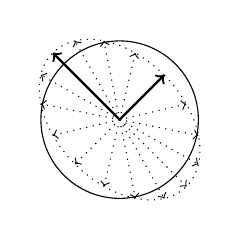
\begin{tikzpicture}
        \draw (0,0) circle (1);
        \draw[rotate=45,dotted] (0,0) ellipse (0.8 and 1.2);
        \draw[rotate=45,thick,->] (0,0) -- (0.800,0.000);
        \draw[rotate=45,dotted,->] (0,0) -- (0.739,0.459);
        \draw[rotate=45,dotted,->] (0,0) -- (0.566,0.849);
        \draw[rotate=45,dotted,->] (0,0) -- (0.306,1.109);
        \draw[rotate=45,thick,->] (0,0) -- (0.000,1.200);
        \draw[rotate=45,dotted,->] (0,0) -- (-0.306,1.109);
        \draw[rotate=45,dotted,->] (0,0) -- (-0.566,0.849);
        \draw[rotate=45,dotted,->] (0,0) -- (-0.739,0.459);
        \draw[rotate=45,dotted,->] (0,0) -- (-0.800,0.000);
        \draw[rotate=45,dotted,->] (0,0) -- (-0.739,-0.459);
        \draw[rotate=45,dotted,->] (0,0) -- (-0.566,-0.849);
        \draw[rotate=45,dotted,->] (0,0) -- (-0.306,-1.109);
        \draw[rotate=45,dotted,->] (0,0) -- (-0.000,-1.200);
        \draw[rotate=45,dotted,->] (0,0) -- (0.306,-1.109);
        \draw[rotate=45,dotted,->] (0,0) -- (0.566,-0.849);
        \draw[rotate=45,dotted,->] (0,0) -- (0.739,-0.459);
      \end{tikzpicture}
      \caption{After} \label{fig:genre-after}
  \end{subfigure}
\end{figure}

It's another Hermitian operator, so it has again picked out two orthogonal directions along which it only applies a scaling.

There is no "true" basis against which a state vector is actually supposed to be measured. Basis vectors are just states that have a particular significance for certain operators.

\begin{figure}[h]
  \centering
    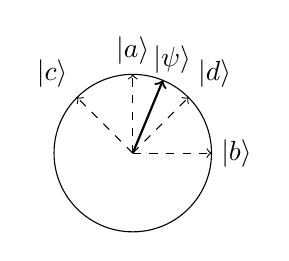
\begin{tikzpicture}
      \draw (0,0) circle (1);
      \draw[thick,->] (0,0) -- (0.383,0.924);
      \node at (0.500,1.190) {$|\psi\rangle$};
      \draw[dashed,->] (0,0) -- (1,0) node[anchor=west] {$|b\rangle$};
      \draw[dashed,->] (0,0) -- (0,1) node[anchor=south] {$|a\rangle$};
      \draw[dashed,->] (0,0) -- (-0.707,0.707) node[anchor=south east] {$|c\rangle$};
      \draw[dashed,->] (0,0) -- (0.707,0.707) node[anchor=south west] {$|d\rangle$};
    \end{tikzpicture}
  \centering
  \caption{No special basis} \label{fig:state-no-special-basis}
\end{figure}

The state could be aligned with $|a\rangle$, so the genre would be uncertain, and then it could become aligned with $|c\rangle$ and then the mood would be uncertain.

To relate all this back to more realistic QM scenarios:

\begin{itemize}
  \item instead of restricting to real scalars, we allow complex scalars,
  \item as well as just two orthogonal directions in state space, we allow infinitely many, even a continuum (as with position and momentum),
  \item we use the Hermitian inner product, taking the complex conjugate on the left, which means that the inner product of a vector with itself will always be real and positive, but the inner product between two different vectors may be complex,
  \item operators cannot generally be represented by matrices due to the continuous nature of some state spaces, but where they can, the matrix is Hermitian or self-adjoint, meaning that it is equal to its own conjugate transpose, which is the complex equivalent of a symmetric matrix,
  \item orthogonal eigenvectors of a Hermitian operator may in some cases have the same eigenvalue, and thus represent states that cannot be distinguished between by means of a measurement of the observable (picture our circle of state vectors growing or shrinking uniformly in all directions and thus remaining a circle, instead of being distorted into an ellipse),
  \item to get a probability from a complex coordinate, we take the modulus squared, to ensure it's a real number.
\end{itemize}

\section{Time Independent Potentials}

In the Schrödinger equation, if the potential $V$ is constant everywhere (and thus may as well be zero everywhere), it reduces to the free particle equation that fell out automatically from the fact that kinetic energy is tied to momentum. A real particle wave function will be some shape that is smooth, differentiable and vanishes at infinity, but it nevertheless always be thought of as the sum of an infinite set of contributing simple corkscrew waves, which means its behaviour is entirely predictable from a time-independent snapshot of the wave $\psi(x)$.

If the potential is a more interesting function it gets trickier. To understand the effect of varying $t$ and $x$ separately, we can suppose the existence of two functions $\psi(x)$ and $\phi(t)$ that when multiplied give us $\Psi(x, t)$.

It is not generally true that this is possible. Even something as simple as $\Psi(x, t) = x + t$ can't separated into a product of two functions of $x$ and $t$. It's obviously true that solutions to the zero-potential Schrödinger equation can be separated, simply because we obtained it from the assumption:

$$
\Psi(x, t) = \exp \left[ {\frac{i(px - Et)}{\hbar}} \right]
$$

which can easily be written as the product of two separate functions of $x$ and $t$:

$$
= \exp \left[ {\frac{ipx}{\hbar}} \right]
\exp \left[ {\frac{-iEt}{\hbar}} \right]
$$

But when a potential is included, and it is some complex function of $x$ and $t$, that is no longer necessarily possible. But we can still discover some useful things by assuming the potential does not depend on $t$, and that is an acceptable approximation. So the whole time-dependent wave function is a product of two parts:

$$\Psi(x, t) = \psi(x) \phi(t)$$

Taking partials becomes ordinary differentiation, because the other factor is constant:

$$
\frac{\partial \Psi}{\partial t}
= \psi \frac{d \phi}{d t},
\frac{\partial^2 \Psi}{\partial x^2}
= \frac{d^2 \psi}{d x^2}  \phi
$$

So we just plug those into \eqref{eqn:se}:

$$
i\hbar
\psi \frac{d \phi}{d t}
=
- \frac{\hbar^2}{2m}
\frac{d^2 \psi}{d x^2}  \phi
+ V \psi \phi
$$

Dividing by $\psi \phi$:

$$
i\hbar
\frac{1}{\phi}
\frac{d \phi}{d t}
=
- \frac{\hbar^2}{2m}
\frac{d^2 \psi}{d x^2}
\frac{1}{\psi}
+ V
$$

To make this explicit, let's put the parameters on each function:

$$
i\hbar
\frac{1}{\phi(t)}
\frac{d \phi(t)}{d t}
=
- \frac{\hbar^2}{2m}
\frac{d^2 \psi(x)}{d x^2}
\frac{1}{\psi(x)}
+ V(x)
$$

The LHS only depends on $t$, the RHS only depends on $x$ (this wouldn't have worked without the simplifying assumption that $V$ is independent of $t$). This means if we hold $x$ constant, and therefore the RHS constant, this equation still holds even if we vary $t$! And of course vice versa. Which means both sides are equal to the same constant, which we will call $E$ for a good reason (spoilers!)

Equating the LHS with $E$:

$$
i\hbar
\frac{1}{\phi}
\frac{d \phi}{d t}
= E
\therefore
\frac{d \phi}{d t}
=
- \frac{Ei}{\hbar}
\phi
\therefore
\phi = e^{-iEt/\hbar}
$$

The RHS isn't so neat, but:

$$
- \frac{\hbar^2}{2m}
\frac{1}{\psi}
\frac{d^2 \psi}{d x^2}
+ V
=
E
\therefore
- \frac{\hbar^2}{2m}
\frac{d^2 \psi}{d x^2}
+ V\psi
=
E\psi
$$

Solutions for $\psi$ will depend on $V$ of course. But the whole wave function is therefore:

$$\Psi(x, t) = \psi(x) e^{-iEt/\hbar}$$

Why is this interesting? Because the more complicated space-sensitive part is frozen w.r.t. time, we can understand the time evolution by just looking at the extremely simple factor:

$$
e^{-iEt/\hbar}
$$

Whatever the solution to $\psi$, the complex value of every point in space is only changing by the above factor as time passes.

And that factor is really just $e^{i\theta}$ with the angle being $-Et/\hbar$, so we know the modulus of the value isn't changing; it's just going "round and round" clockwise in the complex plane.

And if the modulus isn't changing, the probability density isn't changing, so the particle isn't moving. Hence solutions of this type are known as \textit{stationary states}. The expectation value of the position is fixed, and so all other observables' expectation values are also constant, including energy.

The shape of a stationary state, as defined by the $x$-dependent factor, is a fixed structure which never deforms, but just tumbles over and over as time passes, like it's rotating on a spit, although the rate of rotation has $\hbar$ on the bottom of the fraction, which is about $10^-34$, so it's rotating extremely quickly.

\section{Bound States}

When we constructed the Schrödinger equation \eqref{eqn:se} we did so by building an expression for the total energy in terms of the particle's kinetic energy and a potential:

$$
- \frac{\hbar^2}{2m} \frac{\partial^2 \Psi}{\partial x^2} + V{\Psi}
$$  

Comparing this to our RHS differential equation:

$$
- \frac{\hbar^2}{2m}
\frac{d^2 \psi}{d x^2}
+ V\psi
=
E\psi
$$

So in one of these stationary states, $\psi$ substitutes for $\Psi$, which is quite valid because the energy is constant, and so it's the same expression. We can extract an operator for the energy (the Hamiltonian):

$$
\hat{H} = 
- \frac{\hbar^2}{2m} \frac{\partial^2}{\partial x^2} + V
$$

And in a stationary state, it's just:

$$
\hat{H}\psi
=
E\psi
$$

This is an eigenvalue equation: for some solutions $\psi$, the $\bar{H}$ operator has the same effect as multiplying by a constant, the energy eigenvalue $E$ for that $\psi$. It can be shown that it's a Hermitian operator, so the eigenvectors for stationary states with distinct energy eigenvalues can be used to define an orthonormal basis.

Note that we're not talking about a single general operator for all situations. The definition of $V(x)$ will depend on the situation, and that will affect the solutions of the above eigenvalue equation.

There are several standard potentials that can be analysed in this way. The simplest is the infinite square well, a potential that is zero in a small region of width $a$ but infinite outside that region, forcing the wave function to be zero at the boundaries of the region and causing it to have eigenfunctions that are standing waves:

$$
\psi_n(x) =
\sqrt{\frac{2}{a}} sin \lparen \frac{n\pi}{a} x\rparen
$$

with corresponding energy eigenvalues:

$$
E_n = \frac{n^2\pi^2\hbar^2}{2ma^2}
$$

The interesting thing about this is that the set of eigenfunctions, while infinite, is a countable infinity: there is a first state, a second state and so on. Despite this, by choosing an infinite subset of these states and summing them, we can generate any function. Strictly speaking, we can generate any periodic function that is zero at the boundaries, but the distinction between periodic and non-periodic functions is irrelevant if we have defined the value to be zero everywhere outside those boundaries; the shape of one cycle of a periodic function can be anything we like.

So there is no limit on what the initial state can be, but by decomposing that $t = 0$ state $\Psi(x, 0) = \psi(x)$ into a sum of these discrete waves, we know exactly how it will evolve over time. Each component eigenfunction evolves due to the "round and round" factor $e^{-iEt/\hbar}$. Because we're adding complex values at each point in space, even though those component values each have a time-independent modulus, the sum of them does not (think of a clock hand with another clock hand on the end of it, running at different rates). So this is a way to make non-stationary solutions. Wave packets that "move" can be composed by summing stationary states that do not. A particle confined inside a potential can be in a stationary state, or it can "slosh" from side to side in a complicated way due to being a linear combination of many such states.

So we have an exact solution for how any initial state will evolve inside an infinite well potential, assuming the total energy is constant. The energy, by definition, is the quantity that is preserved as time passes, and that's why energy eigenfunctions are of primary importance in analysing the time evolution of a system. To get an exact expression for the wave function as a function of time, we resolve it into a sum of energy eigenfunctions, each of which has its time evolution entirely determined by the factor $e^{-iEt/\hbar}$.

The energy eigenfunctions serve as a set of basis vectors. Why? Because the energy operator is Hermitian, so among its eigenvectors, any two that corresponding to distinct eigenvalues will be orthogonal. For stationary states $m$ and $n$:

$$
\int
\psi_m^* \psi_n dx = \delta_{nm}
$$

This does not mean that $\psi_m^* \psi_n$ is zero everywhere if $m \ne n$, but it does mean that for every non-zero value pointing in some direction in the complex plane, there's another value of the same modulus pointing the opposite way, to balance it out.

So each possible energy value is represented by an eigenvector. We can create a weighted sum of them to make any possible state. We can use those weightings as the components of a vector describing a state. That is, the state of the lowest energy level is a column vector of numbers where the first component is $1$ (or some complex number of modulus $1$) and all the other components are $0$.

There are two complications to this story:

\begin{itemize}
  \item In some situations we find that multiple eigenvectors have the same eigenvalue, so we cannot infer the state vector from an energy measurement, a predicament known as \textit{energy degeneracy}. We never see this for energy in one dimension of physical space, but in two or three it is unavoidable. Motion back and forth along the x-axis is physically different from such motion along the y-axis, but may be so similar as to require the same energy.
  \item We can't measure the energy with absolute precision anyway. No system ever really collapses so its state vector is known to be precisely one of the eigenvectors of whatever observable is being measured. It always remains a superposition to some extent.
\end{itemize}

States where the particle is trapped in a potential are known as \textit{bound states}. In the absence of a potential, particles are in \textit{scattering states}, where the possible energies are not quantised but continuous, so we have to use an integral to find the inner product:

$$
\langle \alpha | \beta \rangle
=
\int
\alpha^* \beta \,dx
$$

If we knew a particle's exact location, $\alpha$, our wave function of space $\psi(x)$ would have a single spike where $x = \alpha$ and be zero everywhere else. Alternatively if knew its exact momentum (and $p=h/\lambda$) our wave function would be a wave with a single wavelength. So we're dealing with Fourier transforms. At these extremes of certainty/uncertainty, one domain has a simple wave of infinite extent, and the other domain has a spike representing that wave. It works either way round.

Thus far we've been working in "position space", using functions of $x$, but alternatively we could work in "momentum space", where the functions are $\phi(p)$. If we knew a particle's exact momentum, $\phi(p)$ would be a spike, whereas if we knew its exact position, $\phi(p)$ would be a single-component wave.

\section{Energy Degeneracy}

Given two eigenvectors of an Hermitian operator, if they have different eigenvalues then they are orthogonal (intuitively they can't be colinear because a linear operator can't apply a different scaling to vectors that are colinear). But what about the converse? If they are orthogonal do they necessarily have different eigenvalues?

Given two eigenstates of the energy operator, $\psi_1$ and $\psi_2$, when we apply the operator it just scales them each by their own eigenvalue:

$$\hat{E}\psi_1 = E_1\psi_1$$
$$\hat{E}\psi_2 = E_2\psi_2$$

If $E_1 \ne E_2$, the two states must be orthogonal. What if we sum the two states and apply the energy operator to the result? The operator is linear, so applying it to a sum of states is the same as applying it to the states separately and then summing the result:

$$\hat{E}(\psi_1 + \psi_2) = \hat{E}\psi_1 + \hat{E}\psi_2 = E_1\psi_1 + E_2\psi_2$$

So the result is a linear combination of the two states. If $E_1 \ne E_2$, this result is not   some single constant $E_3$ multiplied by the sum of the states:

$$\hat{E}(\psi_1 + \psi_2) \ne E_3 (\psi_1 + \psi_2)$$

But if $E_1 = E_2$, then we can pull out a single constant (let's use $E_1$):

$$\hat{E}(\psi_1 + \psi_2) = E_1 (\psi_1 + \psi_2)$$

In other words, any two eigenstates with the same eigenvalue can be added to get a third eigenstate. Obviously this is also true for any linear combination using weightings $a, b$, simply because if $\psi$ is an eigenstate then so is $a\psi$:

$$\hat{E}(a\psi_1 + b\psi_2) = \hat{E}a\psi_1 + \hat{E}b\psi_2 = E_1a\psi_1 + E_2b\psi_2 = E_1(a\psi_1 + b\psi_2)$$

So this is a subspace of the whole vector space, a set of eigenvectors with the same eigenvalue, known (inevitably) as an eigenspace. Any scalar multiple of an eigenvector is also an eigenvector, so the line along which an eigenvector lies is (though not often) called an eigendirection (\textit{eigenalignment} would be a better term), and is the simplest eigenspace that can arise with a linear operator.

In the simple case of a symmetric matrix operating on the plane, it will pick out two orthogonal directions along which it will perform a pure scaling. It may stretch along one direction but squeeze the other. Any vectors colinear with these two directions will only be scaled, their directions unaffected, and thus are eigenvectors. All other vectors will be rotated, and so are not eigenvectors. The set of eigenvectors aligned with one of the directions will all have the same eigenvalue, and so they form an eigenspace.

In QM the magnitude of a state vector is not significant; we always normalise it to a unit vector anyway. Therefore it is truer to say that observable states are represented by eigendirections, and in a given direction we nominate the unit vector to be \textit{the} eigenstate in that direction.

But in the higher dimensional complex vector spaces of QM, some operators will have eigenspaces that are not mere lines, but are themselves multidimensional. That is, there will be a set of vectors that are eigenvectors sharing the same eigenvalue, among which we can find an orthonormal basis of 2 or more dimensions.

The operation of scaling equally in all directions is a trivial example where all vectors are eigenvectors, and all have the same eigenvalue (the scaling factor), so they are all in the same eigenspace, and we can select any N that are not colinear to use as a basis of the N-eigenspace. Suppose we're dealing with a three dimensional vector space, and we scale up by a factor of $1.5$ along the $x$ and $y$ directions, but shrink by $0.5$ along the $z$ direction. A vector aligned with either the $x$ or $y$ direction will be an eigenvector under this scaling operation, with the eigenvalue 1.5. So this is degeneracy: orthogonal eigenvectors with the same eigenvalues, sharing a planar eigenspace that is a proper subset of the whole space.

So while we can say confidently that if two eigenvectors of an Hermitian operator have different eigenvalues then they are orthogonal, we cannot claim the converse: two orthogonal eigenvectors do not necessarily have different eigenvalues. In some circumstances they do, but not all. In particular, by classical intuition, the system of a weight on a string swinging back and forth has a total energy related to the weight's maximum displacement, but it can swing along any axis, so there is an infinite set of states with the same energy. So it is in QM. The inability in some situations to determine the state from the energy is known as degeneracy.

\section{Spin}

Up to this point we've been mostly considering a specific application of the general model of QM, where the classical concepts of position and momentum, which are the building blocks for anything else we might measure, are represented as functions of a continuous variable. The function's value is a complex number that can be mod-squared to get the probability density of that variable. There is something intuitive about this in the space domain, which is why we start with that: it makes us think of an electron as being spread out through space, and having a density that varies. Only when some interaction occurs does it appear to be concentrated entirely at one point. But the momentum of the electron is modelled the same way, and this is not by itself very intuitive. It only becomes a little clearer when we realise that the space representation is a wave, and we can model waves as a sum of simple component waves with a set of frequencies. The momentum function is the Fourier transform of the position function.

But now we're going to consider intrinsic angular momentum. This is introduced to explain how electrons are deflected in a magnetic field, behaviour which is classically suggestive of the electron spinning around an axis, although that physical interpretation seems impossible because the electron's radius (if it is non-zero) is extremely small. Antipodal points on the surface of the electron would have to be moving relative to each other faster than the speed of light. Pauli suggested glossing over this question and just accepting that electrons have an intrinsic angular momentum that cannot be interpreted in some comfortable classical way.

